%texexptitled======================================================================
% lab1-gcd
%-----------------------------------------------------------------------
%

\documentclass[11pt]{article}

% Package includes

\usepackage{graphicx}
\usepackage{color}
\usepackage{comment}
\usepackage{multirow}
\usepackage{askmaps}
\usepackage{amssymb}
\usepackage{amsmath}
\usepackage{tikz}
\usepackage{circuitikzgit}
\usetikzlibrary{arrows, positioning, shapes.geometric, circuits.logic.US}
\tikzstyle{line}=[draw]
\tikzstyle{arrow}=[draw, -latex]

% Wrap long URLs with hyphens
\PassOptionsToPackage{hyphens}{url}\usepackage{hyperref}
\usepackage{pdftexcmds}
\usepackage{upquote}
\usepackage{textcomp}
\usepackage{minted}
\usepackage[listings]{tcolorbox}
\usepackage{enumerate}
\usepackage{enumitem}
\usepackage{mathtools}
\DeclarePairedDelimiter{\ceil}{\Big\lceil}{\Big\rceil}

\tcbset{
texexp/.style={colframe=black, colback=lightgray!15,
         coltitle=white,
         fonttitle=\small\sffamily\bfseries, fontupper=\small, fontlower=\small},
     example/.style 2 args={texexp,
title={Question \thetcbcounter: #1},label={#2}},
}

\newtcolorbox{texexp}[1]{texexp}
\newtcolorbox[auto counter]{texexptitled}[3][]{%
example={#2}{#3},#1}

\setlength{\topmargin}{-0.5in}
\setlength{\textheight}{9in}
\setlength{\oddsidemargin}{0in}
\setlength{\evensidemargin}{0in}
\setlength{\textwidth}{6.5in}

% Useful macros

\newcommand{\note}[1]{{\bf [ NOTE: #1 ]}}
\newcommand{\fixme}[1]{{\bf [ FIXME: #1 ]}}
\newcommand{\wunits}[2]{\mbox{#1\,#2}}
\newcommand{\um}{\mbox{$\mu$m}}
\newcommand{\xum}[1]{\wunits{#1}{\um}}
\newcommand{\by}[2]{\mbox{#1$\times$#2}}
\newcommand{\byby}[3]{\mbox{#1$\times$#2$\times$#3}}


\newenvironment{tightlist}
{\begin{itemize}
 \setlength{\parsep}{0pt}
 \setlength{\itemsep}{-2pt}}
{\end{itemize}}

\newenvironment{titledtightlist}[1]
{\noindent
 ~~\textbf{#1}
 \begin{itemize}
 \setlength{\parsep}{0pt}
 \setlength{\itemsep}{-2pt}}
{\end{itemize}}

% Change spacing before and after section headers

\makeatletter
\renewcommand{\section}
{\@startsection {section}{1}{0pt}
 {-2ex}
 {1ex}
 {\bfseries\Large}}
\makeatother

\makeatletter
\renewcommand{\subsection}
{\@startsection {subsection}{1}{0pt}
 {-1ex}
 {0.5ex}
 {\bfseries\normalsize}}
\makeatother

% Reduce likelihood of a single line at the top/bottom of page

\clubpenalty=2000
\widowpenalty=2000

% Other commands and parameters

\pagestyle{myheadings}
\setlength{\parindent}{0in}
\setlength{\parskip}{10pt}

% Commands for register format figures.

\newcommand{\instbit}[1]{\mbox{\scriptsize #1}}
\newcommand{\instbitrange}[2]{\instbit{#1} \hfill \instbit{#2}}

\graphicspath{{./figs/}}


%-----------------------------------------------------------------------
% Document
%-----------------------------------------------------------------------

\begin{document}
\def\PYZsq{\textquotesingle}


\newcommand{\headertext}{EE240B HW 1}
\renewcommand{\thesubsection}{\thesection.\alph{subsection}}

\title{\vspace{-0.4in}\Large \bf \headertext \vspace{-0.1in}}
\author{Vighnesh Iyer}

\date{\today}
\maketitle

\markboth{\headertext}{\headertext}
\thispagestyle{empty}

\section{HW1}
\begin{enumerate}
\item {\color{blue}For a transistor in strong inversion, the current is dominated by drift rather than diffusion. The channel profile is nevertheless non-uniform which means there is a drift current even in strong inversion. Assuming the square law model (which ignores drift) is a good estimate of the channel charge profile, calculate the diffusion current and compare it to the drift current.}

\item {\color{blue}For your technology DK, what is the compact model used? Which version number? Does the model use binning? If so, by which parameters?}

I'm using GPDK 45nm. The compact model is BSIM v4 based. Binning is done using the $l_{min}, l_{max}, w_{min}, w_{max}$ parameters present in each model. There are 30 different bins for NMOS transistors. Binning changes $V_{th}$-related parameters (like vth0, lvth0, wvth0, pvth0), mobility-related parameters (like u0, lu0, wu0, pu0), subthreshold-related parameters (like voff, lvoff, wvoff, pvoff), and output resistance-related parameters (like pdiblc2, lpdiblc2).

\item {\color{blue}Besides $W$ and $L$, what are the supported instance parameters for your model? Why are detailed layout dependent parameters (such as distance to well edge) used in some models?}

    \begin{itemize}
        \item finger width ($W$)
        \item number of fingers ($W$)
        \item folding threshold (finger width at which to apply device folding in layout)
        \item S/D metal width (width of metal used to short source and drain)
        \item some other ones I don't think matter
    \end{itemize}

    The layout dependent parameters are auto-derived from the basic instance parameters (I guess for the PDK-reference layout of this transistor). These layout dependent parameters can be overridden as instance parameters. These detailed layout parameters can be used to estimate device parasitics at schematic-design time.

\item {\color{blue}Set up a schematic (don't rely on the simulator to output small-signal parameters) and plot the intrinsic gain ($a_{v0}$) of the minimum sized transistor versus $V_{gs}$. Make sure you hold $V_{DS}$ constant (use an ideal op-amp - VCVS) to setup the simulation. Plot the intrinsic gain versus $I_{ds}$ and $V^*$. What is your conclusion? Do you expect a strong bias current dependence? Explain.}

    I'm holding $V_{DS}$ at mid rail = $\frac{1.1}{2}$ and sweeping $I_{ds}$. I'm using a SVT transistor with minimum size ($L_{min} = 45n, W_{min} = 120n$). Here are the plots:

    \begin{figure}[H]
        \centering
        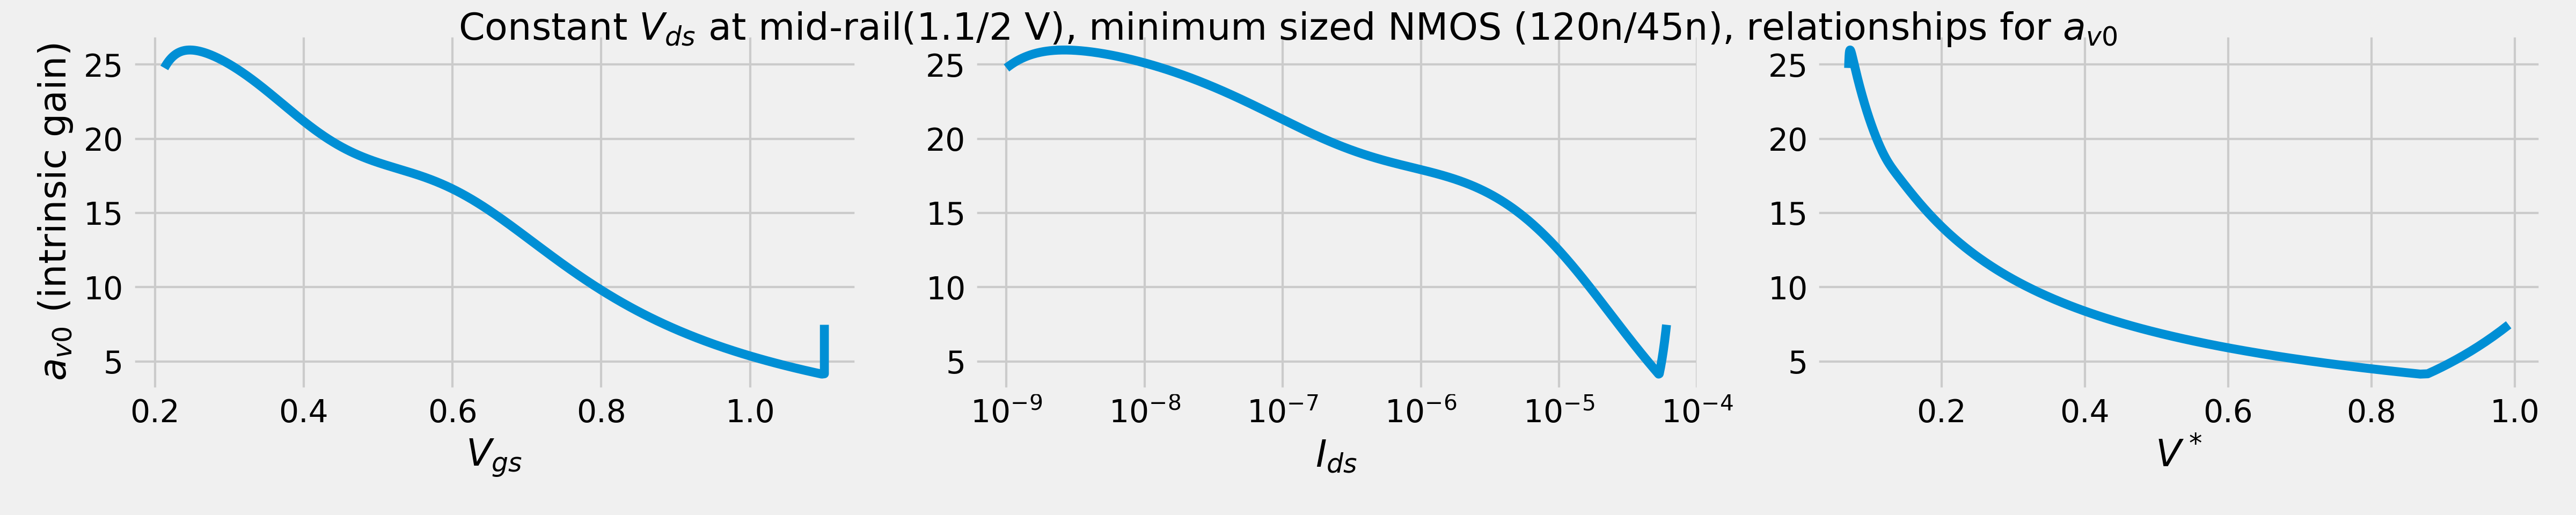
\includegraphics[width=\textwidth]{figs/problem4.png}
    \end{figure}

    \begin{itemize}
        \item $a_{v0}$ has an inverse relationship to drain current $I_{ds}$ (logarathmic) and $V_{gs}$ (linear)
        \begin{itemize}
            \item This is expected because the $r_o$ of the device decreases more rapidly than the $g_m$ increases as $I_{ds}, V_{gs}$ increase.
        \end{itemize}
        \item $a_{v0}$ versus $V^*$, follows the $V_{gs}$ relationship and this is one reason for using the $V^*$ design methodology to choose the transistor's operating point.
    \end{itemize}

\item {\color{blue}Now re-plot the instinsic gain $a_{v0}$ for a few non-minimum length devices. Try $2 L_{min}$, $3 L_{min}$, and $L_{max}$. Does the gain depend on $W$? Explain why you should avoid using a very small $W$. $L_{max}$ is the longest channel length supported by the DK.}

    \begin{figure}[H]
        \centering
        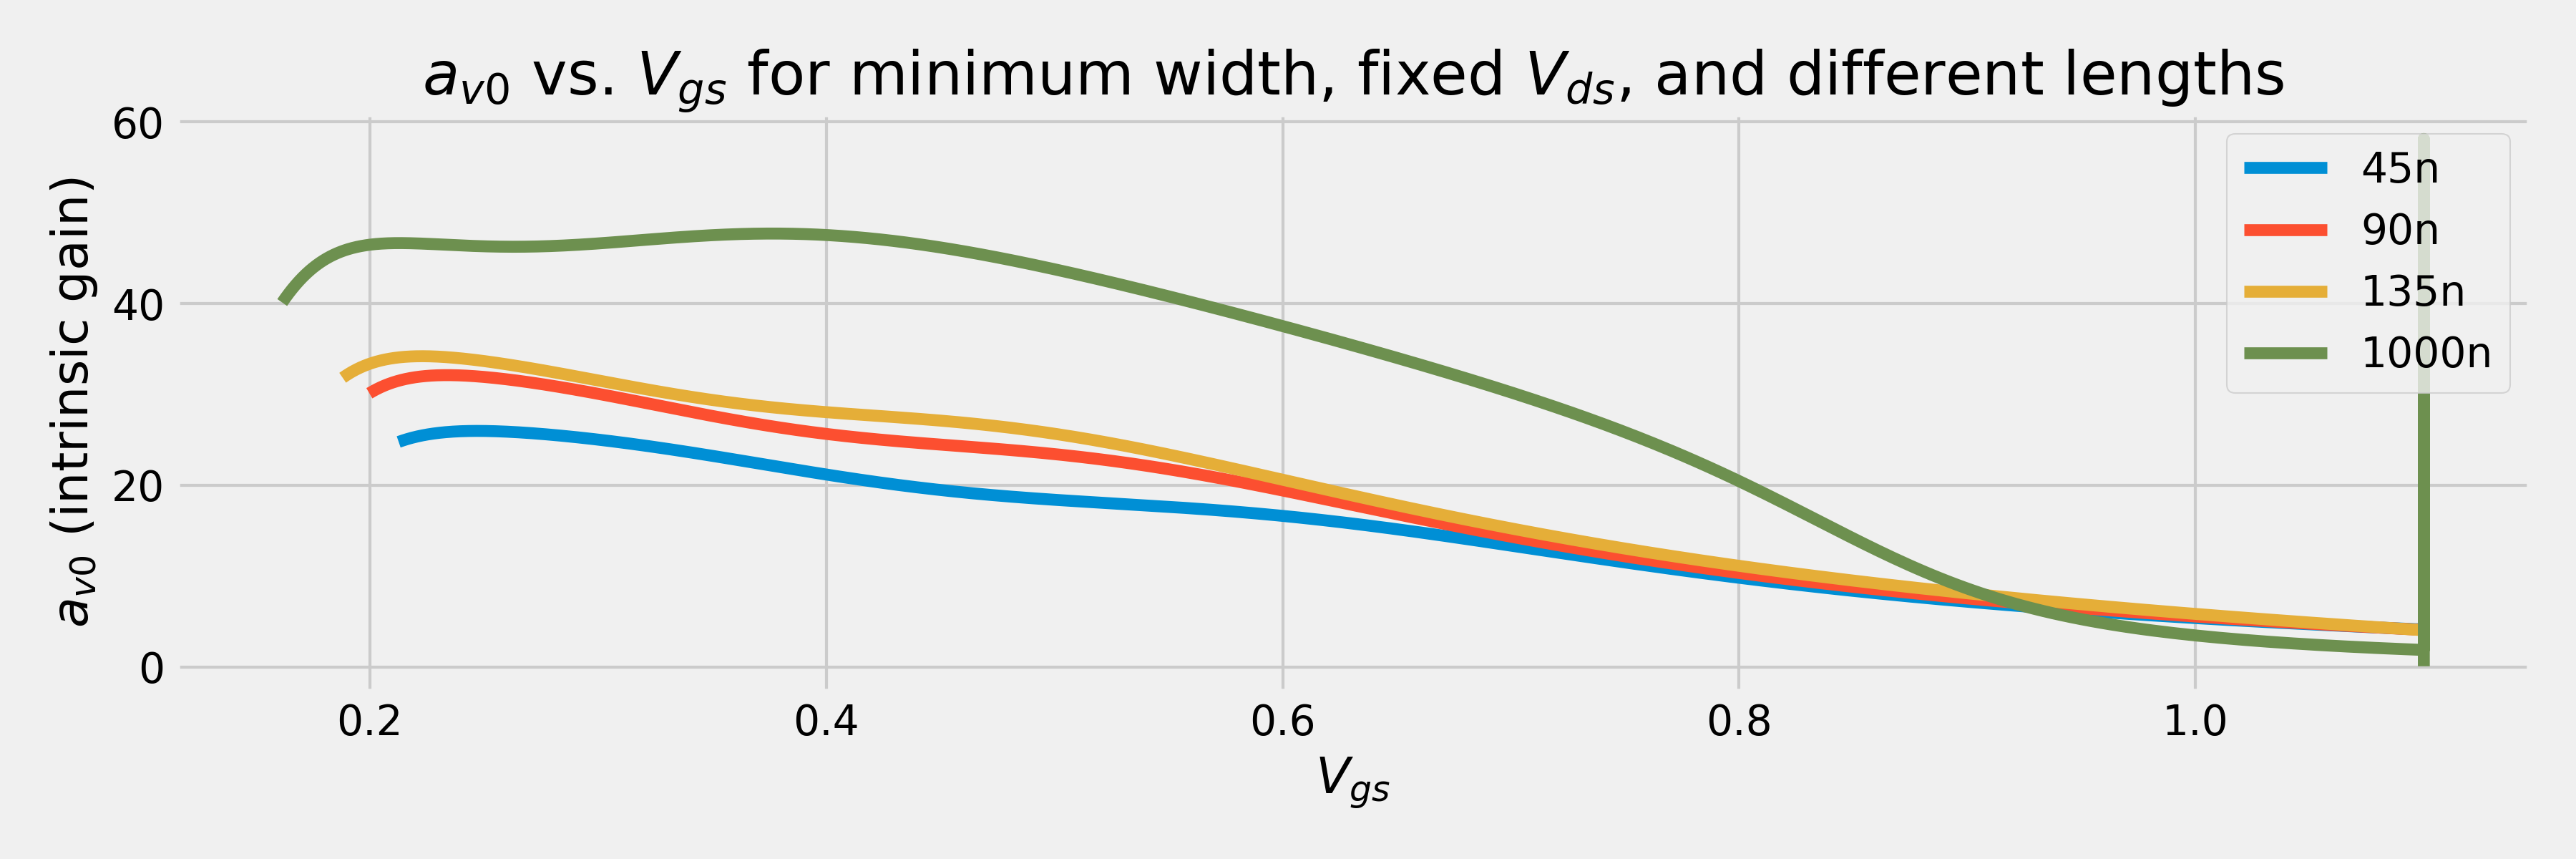
\includegraphics[width=0.8\textwidth]{figs/problem5.png}
    \end{figure}

    In this process $L_{max} = 10 \mu m$, but this gave weird simulation results, so I'm using $L_{max} = 1 \mu m$.
    \begin{itemize}
        \item The intrinsic gain also doesn't depend on $L$ after the transistor is strongly saturated since the $r_o$ vs $g_m$ relationship begins to look similar across lengths.
        \item The intrinsic gain generally doesn't depend on $W$ since $r_o$ and $g_m$ both scale linearly with the transistor width.
        \item A very small $W$ however has a proportionally larger $C_{dd}$ and $C_{gg}$ than a wider transistor, which can lead to significant schematic/layout mismatches post-layout and extraction (and frequency dependent gain differences too).
    \end{itemize}

\item {\color{blue}Which capacitance model does your model use? What is the charge partition scheme?}

    The capacitance model is capmod = 2 (a smooth and single charge (with thickness) equation). The xpart parameter says the charge partition scheme is 0/100.

\item {\color{blue}Setup a simulation to plot the normalized input capacitances seen from the gate ($C_{gs}, C_{gd}, C_{gb}$) of a MOS device as you vary $V_{gs}$ and hold $V_{ds}$ constant in triode and saturation (normalize by $C_{ox}$). Are the expected symmetry properties upholding? Specify as many physical constraints as possible and check to see they are upheld by the model.}

    \begin{figure}[H]
        \centering
        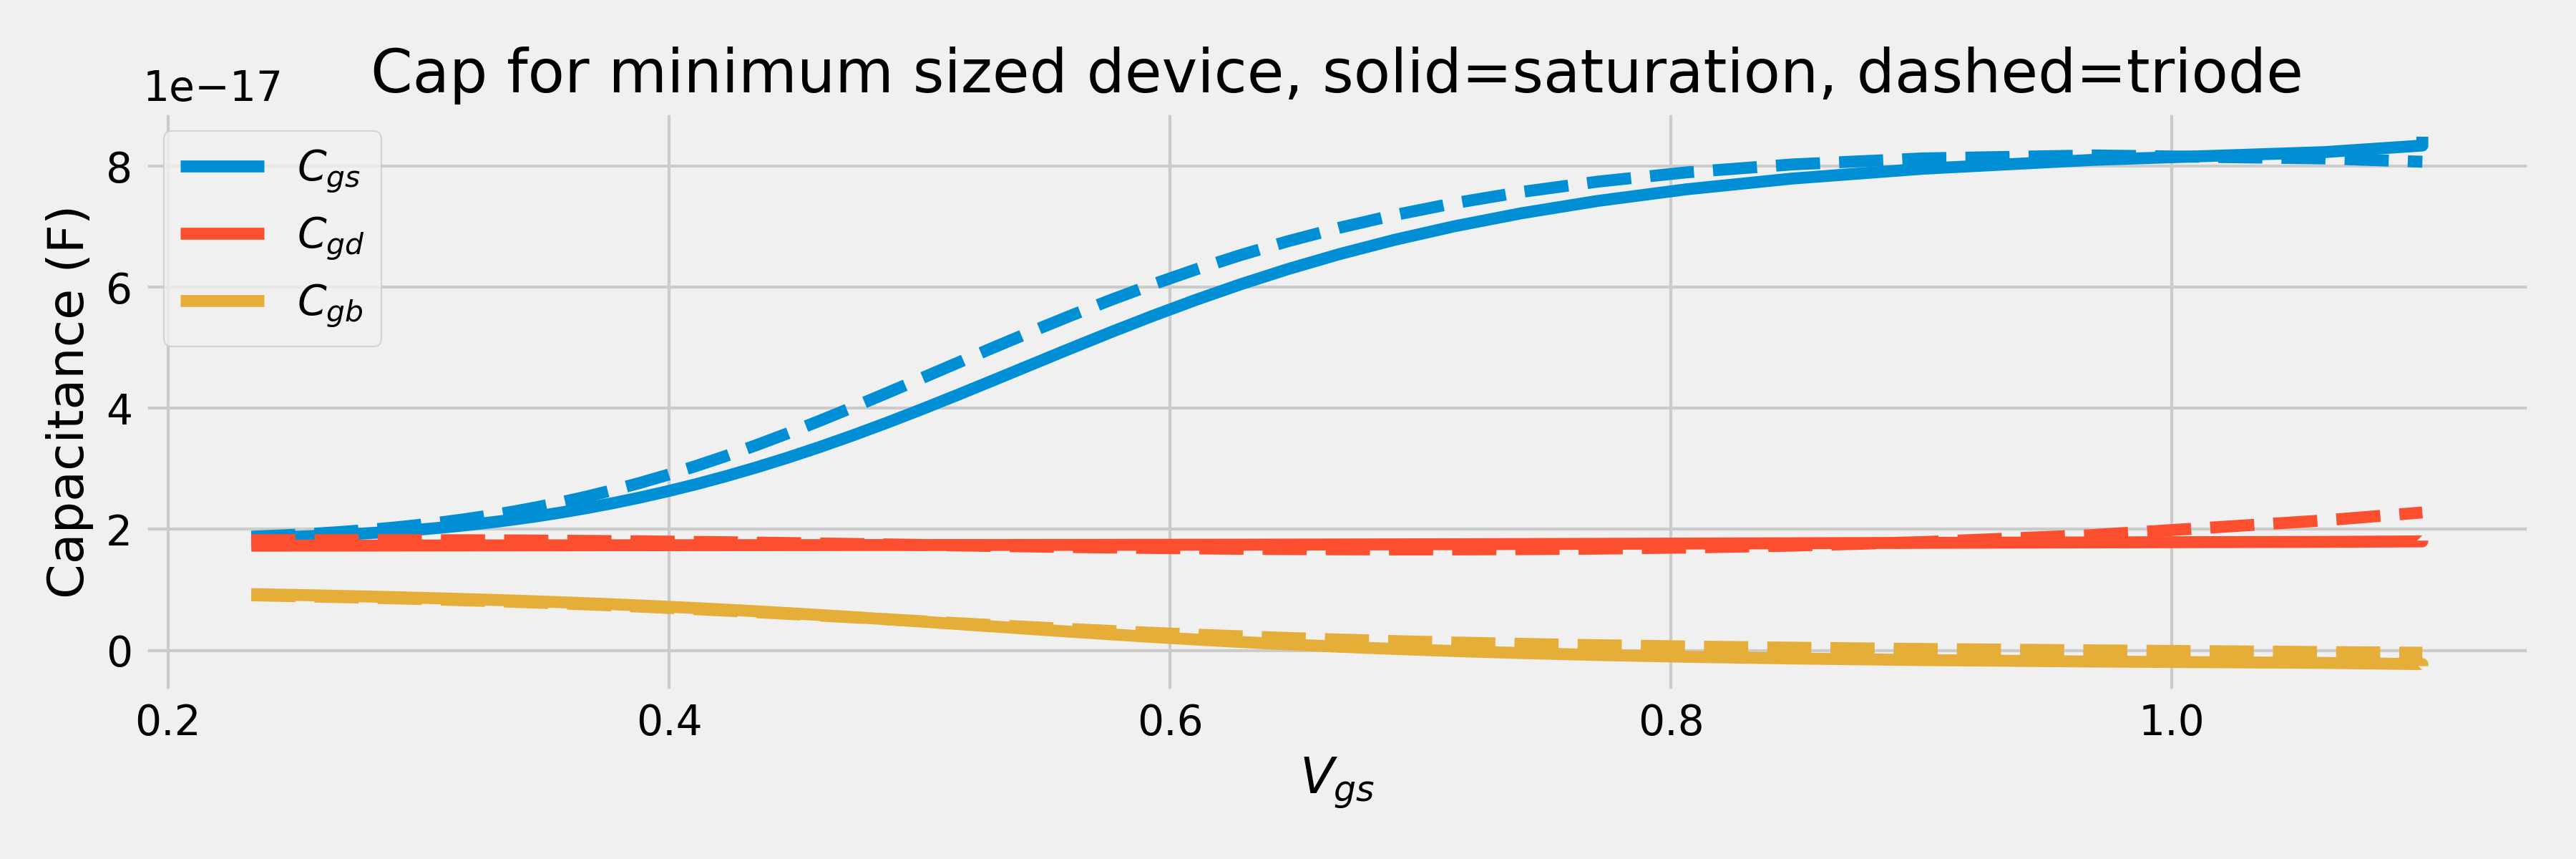
\includegraphics[width=0.8\textwidth]{figs/problem7.png}
    \end{figure}

    The triode $V_{ds} = 0.2 V$ and the saturation $V_{ds} = 0.9 V$. $V_{gs}$ is varied by sweeping $I_{ds}$.

\item {\color{blue}Plot $\frac{g_m}{I_d}$ versus $V_{gs}$ for the minimum, $2 L_{min}$, $3 L_{min}$, and $L_{max}$ of your technology. Superimpose the expected sub-threshold and square-law behavior and compare.}

    \begin{figure}[H]
        \centering
        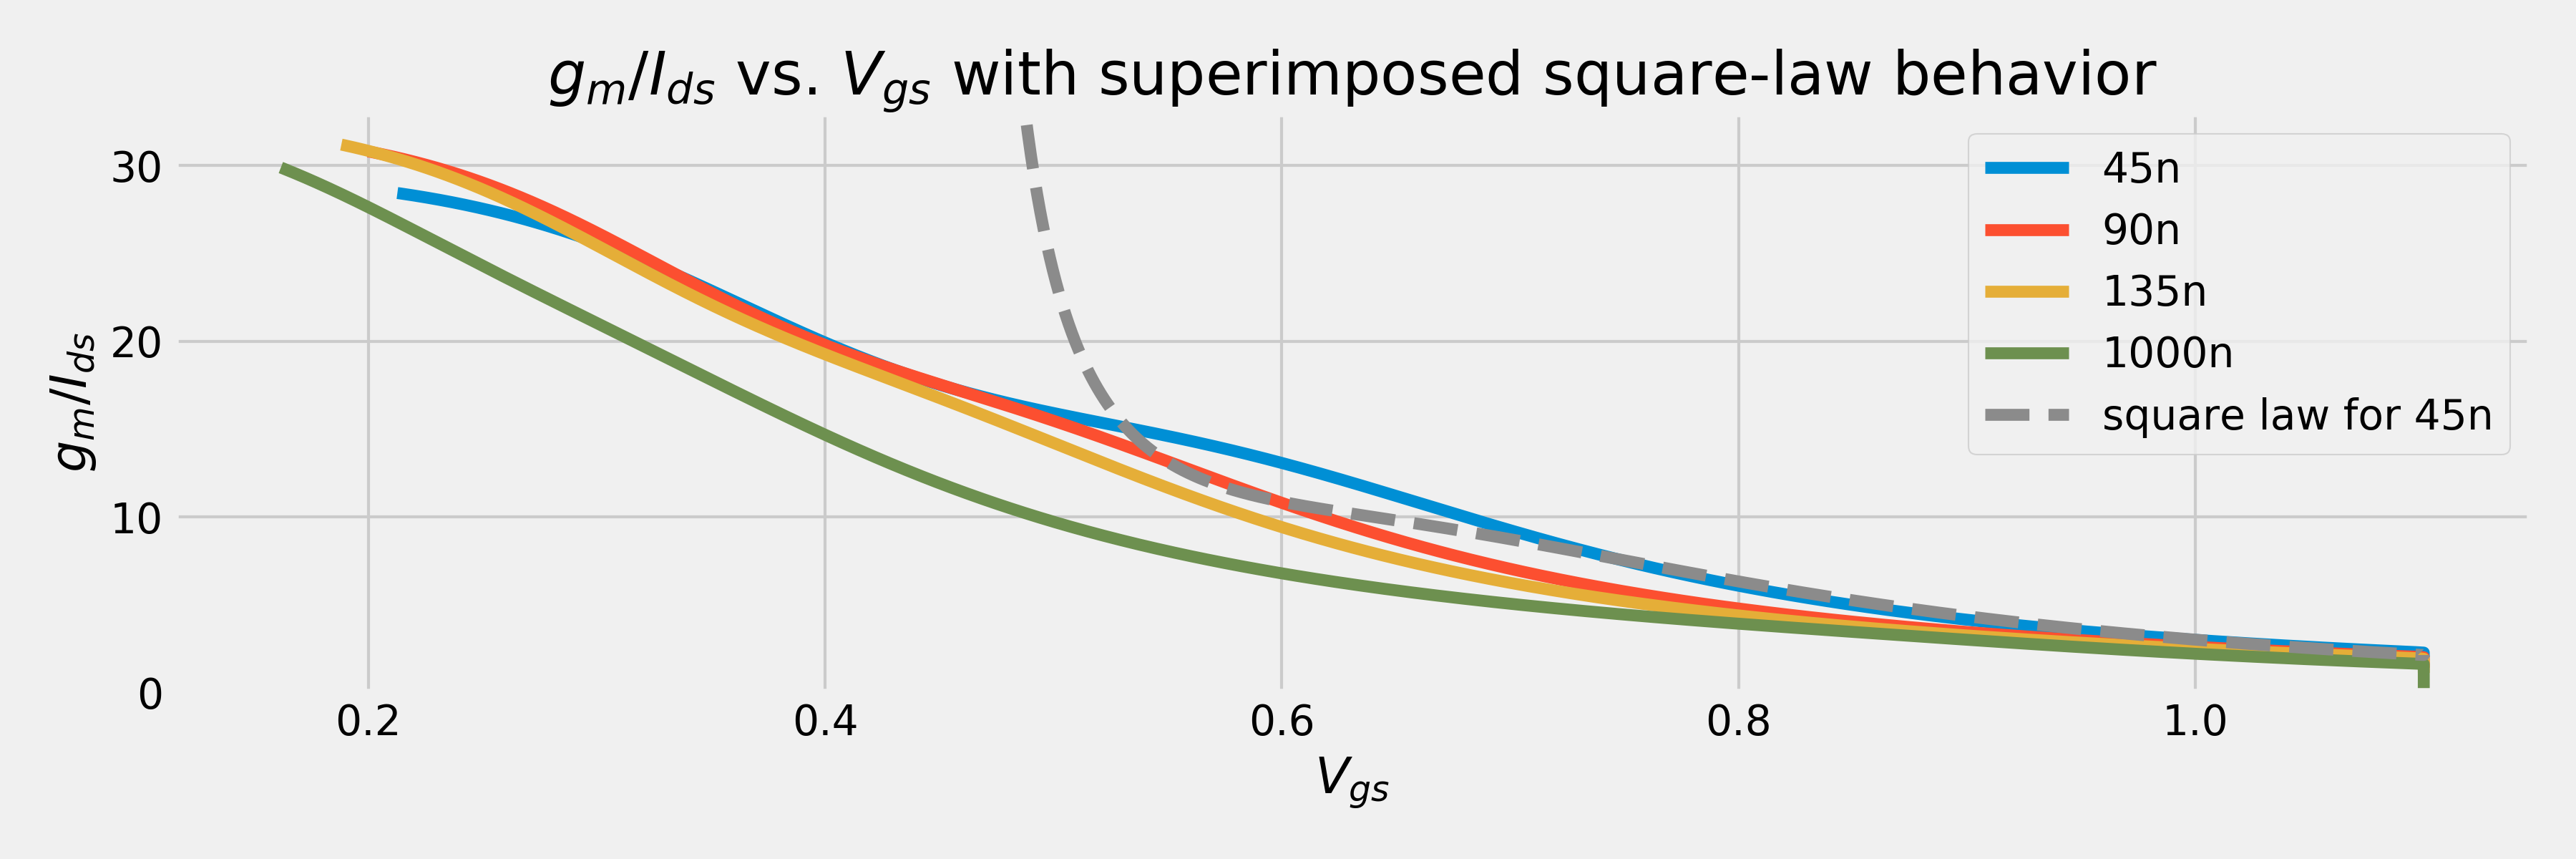
\includegraphics[width=0.8\textwidth]{figs/problem8.png}
    \end{figure}

    I assumed the square law was $I_{ds} = k \frac{W}{L} (V_{gs} - V_{th})^2$, and allowed $k$ and $V_{th}$ to be fitting parameters. I allowed fitting from midway through the $I_{ds}$ sweep.

\item {\color{blue}Plot $V^*$ versus $V_{gs}$ for the minimum, $2 L_{min}$, $3 L_{min}$, and $L_{max}$ of your technology. Superimpose the expected sub-threshold and square-law behavior and compare.}

    \begin{figure}[H]
        \centering
        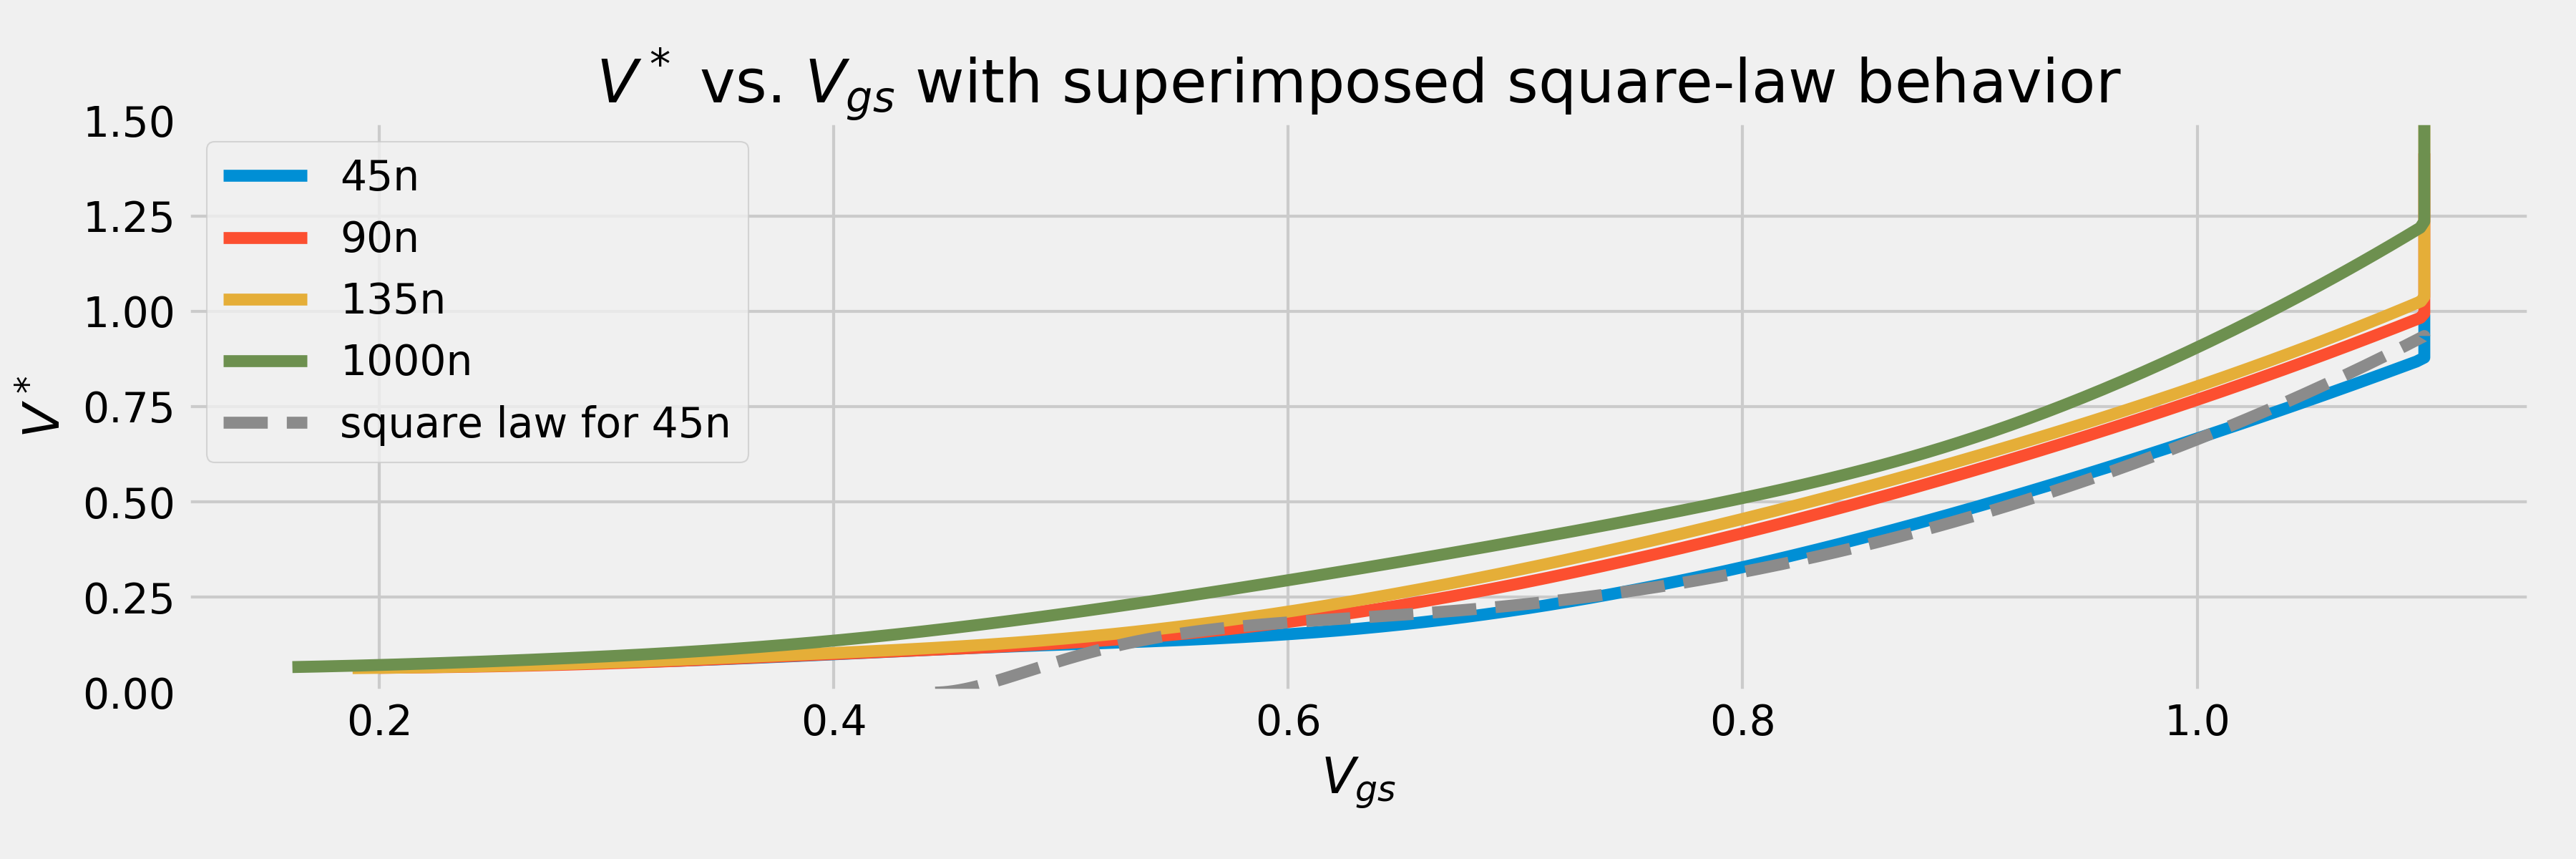
\includegraphics[width=0.8\textwidth]{figs/problem9.png}
    \end{figure}

    I used the same square-law fitting procedure. This curve makes sense since $V^*$ is just an analog for $V_{ov} = V_{gs} - V_{th}$. The curved polynomial behavior indicates that at high $V_{gs}$, $V^*$ is less affected mostly due to velocity saturation.

\item {\color{blue}Plot $f_T$ vs $V^*$. Make sure to set up a schematic to extract $f_T$ rather than using the SS-parameters of the model. Use $L_{min}$, $2 L_{min}$, $3 L_{min}$, and $L_{max}$ of your technology. Explain the trends.}

    \begin{figure}[H]
        \centering
        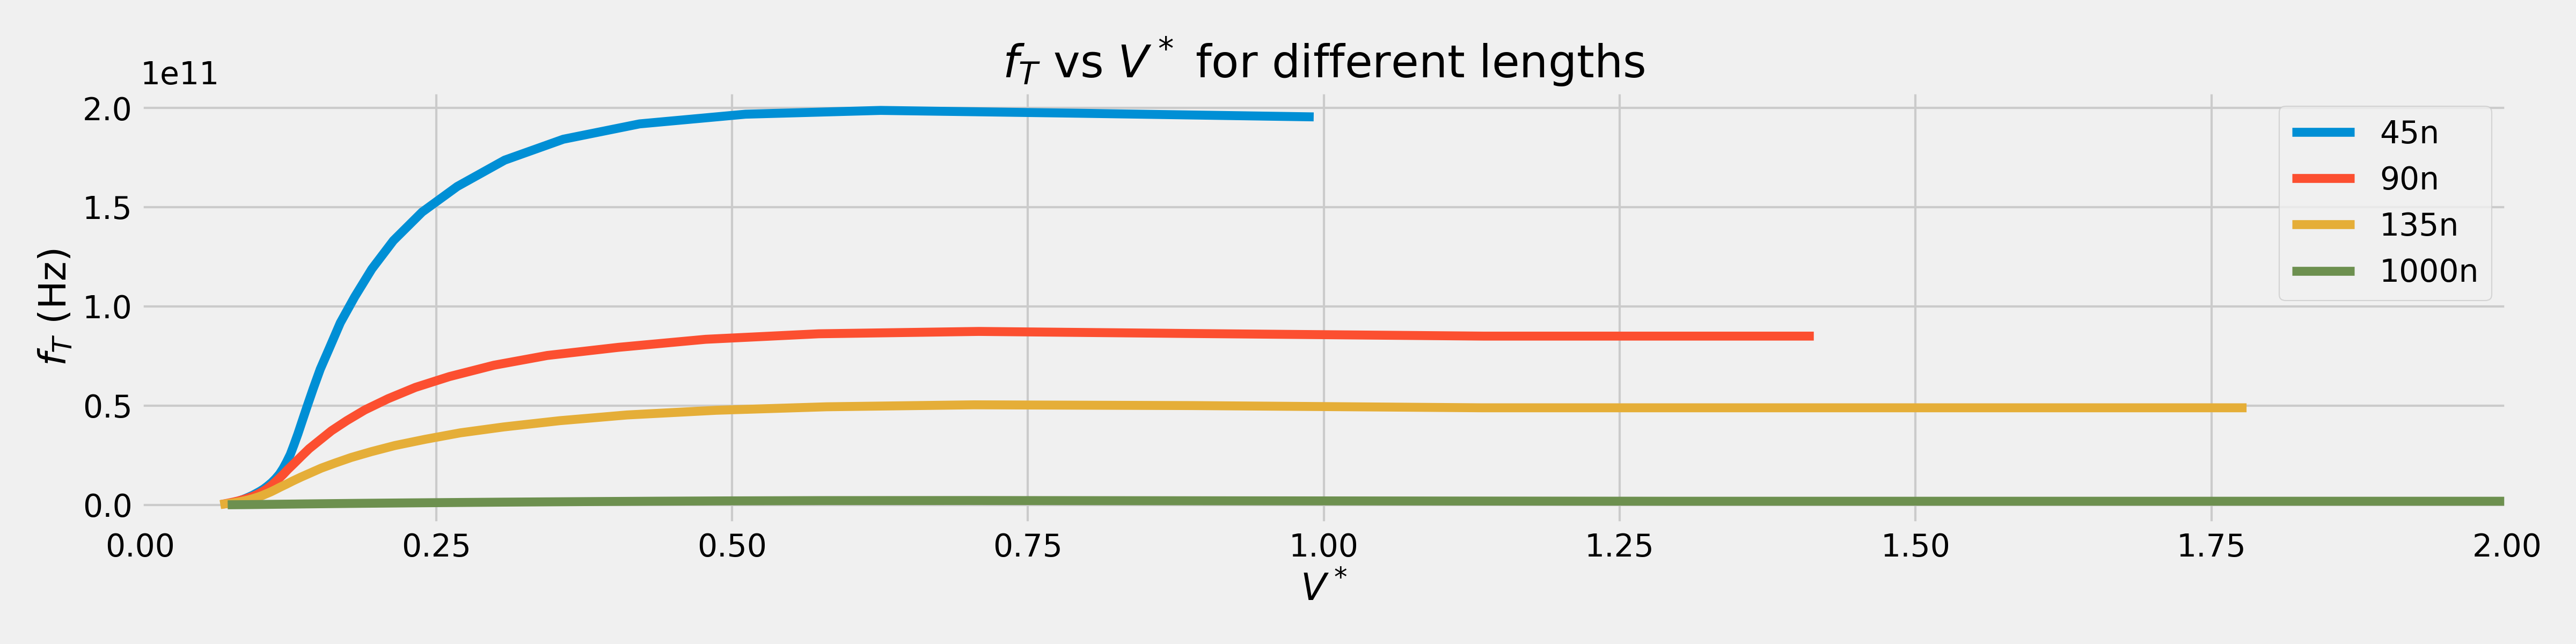
\includegraphics[width=\textwidth]{figs/problem10.png}
    \end{figure}

    I'm extracting $f_T$ for $V_{ds} = 1.1/2 V$ and minimum width of 120n for a SVT NMOS. $I_{ds}$ is swept from 1n to 60u and $V^*$ is derived from correlating this $I_{ds}$ sweep to the previous results obtained. $f_T$ is extracted by analyzing current gain from gate to drain and seeing at what frequency the gain drops to 0dB. Nearly 200 Ghz $f_T$ can be obtained with the minimally sized device in this process.

\item {\color{blue}Plot the product of $f_T$ and $a_{v0}$ vs $V^*$ for $L_{min}$, $2 L_{min}$, $3 L_{min}$, and $L_{max}$. For which $V^*$ is the product maximum for each case?}

    \begin{figure}[H]
        \centering
        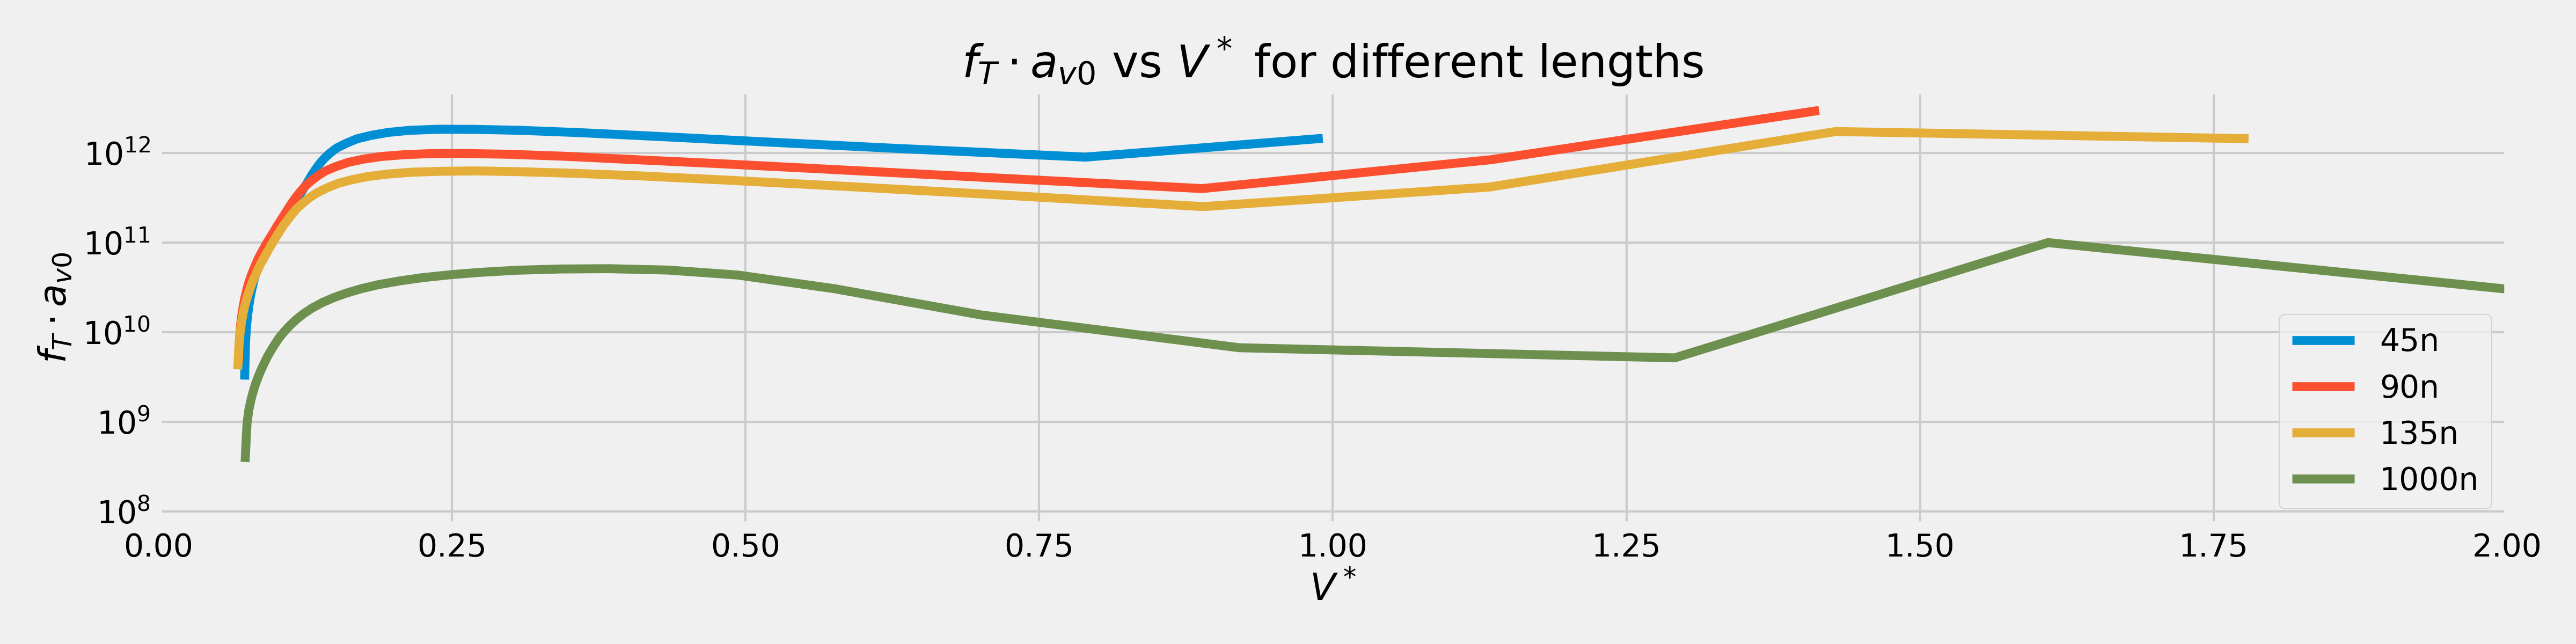
\includegraphics[width=\textwidth]{figs/problem11.png}
    \end{figure}

    The optimal $V^*$ is about 0.23V, 0.25V, 0.27V, 0.375V for the shortest to longest devices.

\item {\color{blue} Design an amplifier that achieves a DC gain of 20 and a unity gain frequency of 500 Mhz while driving a load of 1pF. Specify the required $V^*$, bias current, $V_{gs}$, and device dimensions. Use the results of the previous problems to guide the design choices. Verify with SPICE.}
\end{enumerate}
\end{document}
